%%
% This file is modified based on the LAYOUT_E.TEX provided in REFMAN package. You can find the original REFMAN package at https://ctan.org/pkg/refman. This document only uses the LAYOUT_E.TEX as a template.

%%
% LAYOUT_E.TEX - Short description of REFMAN.CLS
%                                       99-03-20
%
%  Updated for REFMAN.CLS (LaTeX2e)
%
\documentclass[twoside,a4paper]{refart}
\usepackage{makeidx}
\usepackage{ifthen}
% ifthen wird vom Bild von N.Beebe gebraucht!
\usepackage{url}
\usepackage{graphicx}
\usepackage{xcolor}
\usepackage{listings}
\usepackage{csquotes}
\lstset{basicstyle=\ttfamily,
  showstringspaces=false,
  commentstyle=\color{red},
  keywordstyle=\color{blue}
}

\title{Misconduct Detection Project(MDP) Tool\\
Testing and Debugging Report No.2}
\author{Yucheng Xie \\
\today \\
Supervisor: Dr. Kyriakos Kalorkoti\\
Master of Science\\
School of Informatics\\
University of Edinburgh\\
Software Version: 1.0}

\date{}
\emergencystretch1em  %

\pagestyle{myfootings}
\markboth{Testing and Debugging Report No.2}%
         {Testing and Debugging Report No.2}
\makeindex 
\setcounter{tocdepth}{2}

%% Defines the bug name and bug ID here
% =====================================================
\newcommand{\bugfirst}{UI-001: Programming Language Selection Panel}
\newcommand{\bugsecond}{UI-002: Auto Programming Language Selection}
\newcommand{\bugthird}{DET-003: Results Retrieve Error}
\newcommand{\bugfourth}{UI-003: Selection Page Style Loss Error}


\begin{document}

\maketitle

\tableofcontents

\newpage


%%%%%%%%%%%%%%%%%%%%%%%%%%%%%%%%%%%%%%%%%%%%%%%%%%%%%%%%%%%%%%%%%%%%

\section{Summary} \label{sec:intr}
This \enquote{testing and debugging report} is used as a record for later developers referring. Each bug in this report has been illustrated by following three aspects:
\begin{enumerate}
\item The details of the bug. This part is mainly giving the details of the bug, including how to reproduce the bug.
\item The analysis of the bug. This part is mainly focusing on analyzing the bug and providing fixing solutions to the bug.
\item The test cases of the bug. This part is providing the test cases for verifying the bug is resolved.
\end{enumerate}

Especially, in the above information, later developers should always rerun the test cases of a bug if any code related to the bug is changed. Rerunning test cases could guarantee that later changes on the code are not making these bugs recur.

$\ $

Involved bugs in this report:
\begin{enumerate}
\item \bugfirst
\item \bugsecond
\item \bugthird
\item \bugfourth
\end{enumerate}


%% Bug 1
%=====================================================
\section{\bugfirst}
\subsection{Bug Report Part}

\subsection*{General Information}
\begin{table}[!h]
\begin{tabular}{|l|c|}
\hline
\textbf{Title} & Programming Language Selection Panel \\ \hline
\textbf{ID} & (user interface) UI-001 \\ \hline
\textbf{Priority} & Critical \\ \hline
\end{tabular}
\end{table}

\subsection*{Description}
Allow users to decide which detection package and programming language to use. Due to time limitation, this function have not been finished in formal developing stage. Therefore, this function is planned and finished in extra debugging stage. The function in use is shown in Appendix \ref{bug_1_expl}.

\subsection*{How to Reproduce}
Not available.

\subsection*{Screenshots}
See appendix.

$\ $

\subsection{Bug Analysis Part}
Not available.

\subsection{Test Cases Part}
Test Case 1:

\begin{enumerate}
\item Normally upload file and folder, select segments.
\item Provide correct settings, i.e. manually give correct file extension.
\item Perform detection.
\end{enumerate}

Expected Results for this Test Case: 

The results are shown correctly.

$\ $

Test Case 2:

\begin{enumerate}
\item Normally upload file and folder, select segments.
\item Provide incorrect settings, i.e. manually give incorrect file extension.
\item Perform detection.
\end{enumerate}

Expected Results for this Test Case: 

The \enquote{No Results} error page is shown. (details see Appendix \ref{bug_1_expl})

$\ $

Test Case 3:

\begin{enumerate}
\item Register a new detection package in the system.
\end{enumerate}

Expected Results for this Test Case: 

The panel updates the package information and supported programming languages information automatically.

%% Bug 2
%=====================================================
\section{\bugsecond}
\subsection{Bug Report Part}

\subsection*{General Information}
\begin{table}[!h]
\begin{tabular}{|l|c|}
\hline
\textbf{Title} & Auto Programming Language Selection \\ \hline
\textbf{ID} & UI-002 \\ \hline
\textbf{Priority} & Critical \\ \hline
\end{tabular}
\end{table}

\subsection*{Description}
Providing suggestions for users to decide which detection package and programming language to use. Due to time limitation, this function have not been finished in formal developing stage. Therefore, this function is planned and finished in extra debugging stage. The function in use is shown in Appendix \ref{bug_2_expl}.

\subsection*{How to Reproduce}
Not available.

\subsection*{Screenshots}
See appendix.

\subsection{Bug Analysis Part}
Not available.

\subsection{Test Cases Part}
Test Case 1:

\begin{enumerate}
\item Normally upload file and folder, select segments.
\item Provide correct settings, i.e. manually give correct file extension.
\item Perform detection.
\end{enumerate}

Expected Results for this Test Case: 

The results are shown correctly. Nothing else happens.

$\ $

Test Case 2:

\begin{enumerate}
\item Normally upload file and folder, select segments.
\item Provide incorrect settings, i.e. manually give incorrect file extension.
\item Perform detection.
\end{enumerate}

Expected Results for this Test Case: 

The auto selection function open a pop-up window to give the user suggestions about the optimal settings and give warnings to the user. However, if the user insist, auto selection function will follow the user's settings rather than using the optimal settings.

$\ $

Test Case 3:

\begin{enumerate}
\item Normally upload file and folder, select segments.
\item Provide no settings, i.e. manually give no settings to tool.
\item Perform detection.
\end{enumerate}

Expected Results for this Test Case: 

The auto selection function prevent the user from performing detection and open a pop-up window to force the user provide settings.

%% Bug 3
%=====================================================
\section{\bugthird}
\subsection{Bug Report Part}

\subsection*{General Information}
\begin{table}[!h]
\begin{tabular}{|l|c|}
\hline
\textbf{Title} & Results Retrieve Error \\ \hline
\textbf{ID} & DET-003 \\ \hline
\textbf{Priority} & Normal \\ \hline
\end{tabular}
\end{table}

\subsection*{Description}
If the server is shut-down, the result keys will be lost and the user will not be able to retrieve the results. The user will come across a \enquote{key error} when trying to retrieve results.

\subsection*{How to Reproduce}
\begin{enumerate}
\item Perform detection normally.
\item Jump to the \enquote{result page}, it should work correctly.
\item Reboot the server.
\item Jump to the \enquote{result page}, now it should indicates a \enquote{key error}.
\end{enumerate}

\subsection{Bug Analysis Part}
In our tool, we used a \enquote{file name manager} to manage the actual file names and the copied renamed files. However, this \enquote{file name manager} store file relationships in the memory. Therefore, if the server is rebooted or shut down, the file relationships will be lost and thus causes the \enquote{key error}.

Therefore, we store the file relationships on the disk rather than memory to solve this problem.

\subsection{Test Cases Part}
Test Case 1:
\begin{enumerate}
\item Perform detection normally.
\item Jump to the \enquote{result page}, it should work correctly.
\item Reboot the server.
\item Jump to the \enquote{result page} again.
\end{enumerate}

Expected Results for this Test Case: 

The \enquote{result page} should be loaded correctly.

%% Bug 4
%=====================================================
\section{\bugfourth}
\subsection{Bug Report Part}

\subsection*{General Information}
\begin{table}[!h]
\begin{tabular}{|l|c|}
\hline
\textbf{Title} & Selection Page Style Loss Error \\ \hline
\textbf{ID} & UI-003 \\ \hline
\textbf{Priority} & Normal \\ \hline
\end{tabular}
\end{table}

\subsection*{Description}
When refreshing the selection page, the left side highlighted segments will loss their format and become plain text again.

\subsection*{How to Reproduce}
\begin{enumerate}
\item Normally select segments on the \enquote{selection page} and save the selection.
\item Refresh the \enquote{selection page} and all format on the left side should be reset to plain text.
\end{enumerate}

\subsection{Bug Analysis Part}
Here we used a redraw function to redraw the segments when the page is reload. However, the originally highlighted segments got the indexes from the user's selection. In this situation, the user ask to reload the page, the segments cannot obtain the indexes since the user is not highlighting any segment.

To resolve this bug, we decide not to redraw each segment one by one. Instead, we save the HTML file and redraw the whole page. Although this also causes a problem that when we remove any segment, we need to carefully rewrite the HTML page to ensure it is restored to the correct state.


\subsection{Test Cases Part}
Test Case 1:

\begin{enumerate}
\item Normally select segments on the \enquote{selection page} and save the selection.
\item Refresh the \enquote{selection page}.
\end{enumerate}

Expected Results for this Test Case: 

The \enquote{selection page} left side block should be loaded correctly.

Test Case 2:

\begin{enumerate}
\item Remove some segments, add some other segments and save the selections.
\item Refresh the \enquote{selection page}.
\end{enumerate}

Expected Results for this Test Case: 

The \enquote{selection page} left side block should be loaded correctly. The ordering of the segments should be correct. The name of the segments should be correct.

\clearpage

\section*{Appendix}
\addcontentsline{toc}{section}{Appendix}

\appendix

\section{Explanation of Bug Priorities}
In this report, we divided all bugs into three different priority levels. They are:

\begin{enumerate}
\item Critical:

Something could case the whole system to be stopped or case the system producing wrong results.

\item Normal:

Something might affect later developing. Or something might case some further problems if it is not properly resolved.

\item Minor:

Annoying but not harmful to the functionalities. Such as layout displaying error in different browsers.
\end{enumerate}

\section{Programming Language Selection Panel Function in Use}
\label{bug_1_expl}
\begin{figure}[!h]
\centering
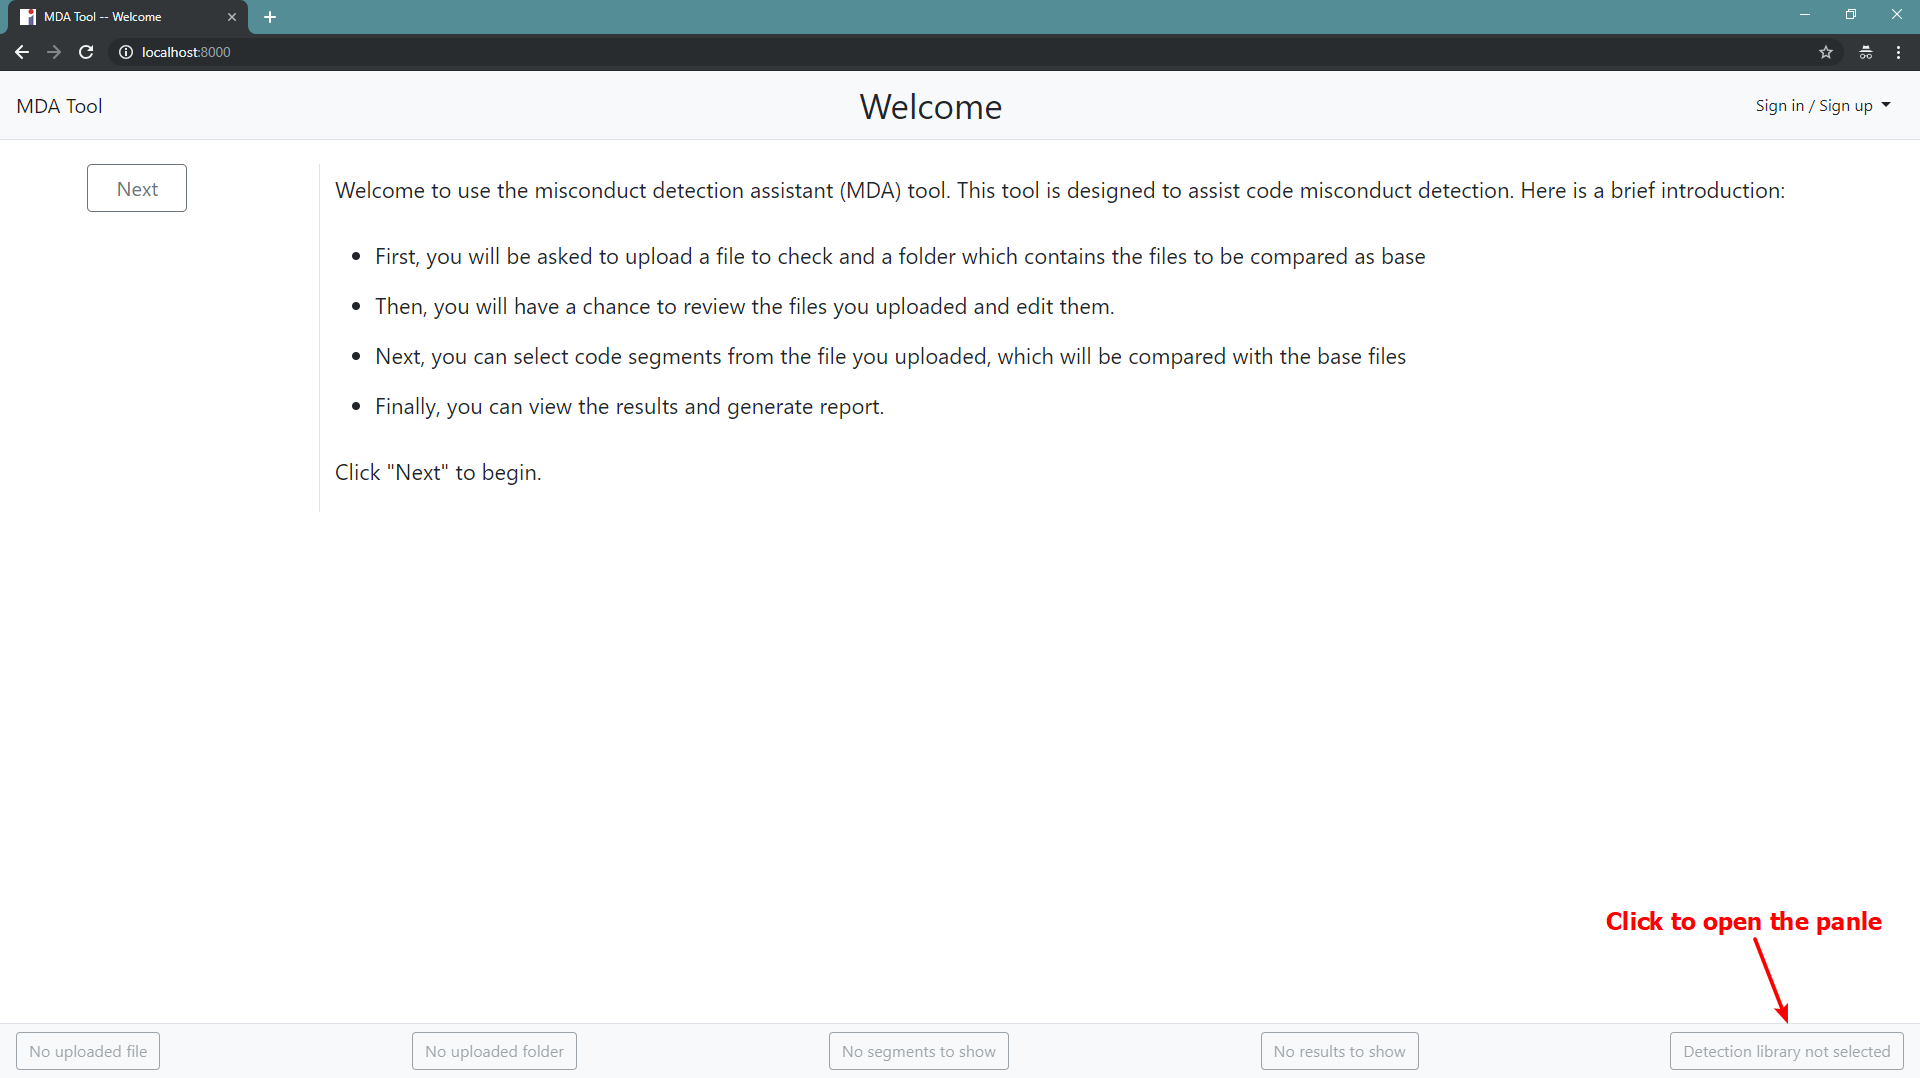
\includegraphics[width=12cm]{img/bug_1-1.png}
\caption{\bugfirst $\ $ Screenshot 1}
\label{fig:bug1_1}
\end{figure}

First, click the highlighted button shown in Figure \ref{fig:bug1_1} to open the selection panel.

Then, the panel will be shown as Figure \ref{fig:bug1_2}.

As shown in Figure \ref{fig:bug1_3}, the user need to first select detection package on the left side. After selected detection package, programming languages supported by the detection package will be shown on the right side. The user need to select one programming language and click \enquote{save changes}

Finally, current settings will be shown at the bottom bar as shown in Figure \ref{fig:bug1_4}.

If the settings go wrong and no results returned (for JPlag, if the settings are incorrect, JPlag will return an empty folder to indicate that), the tool will show a \enquote{No Results} error page to remind the user that the settings might be incorrect. The error page is shown in Figure \ref{fig:bug1_5}.

\begin{figure}[!h]
\centering
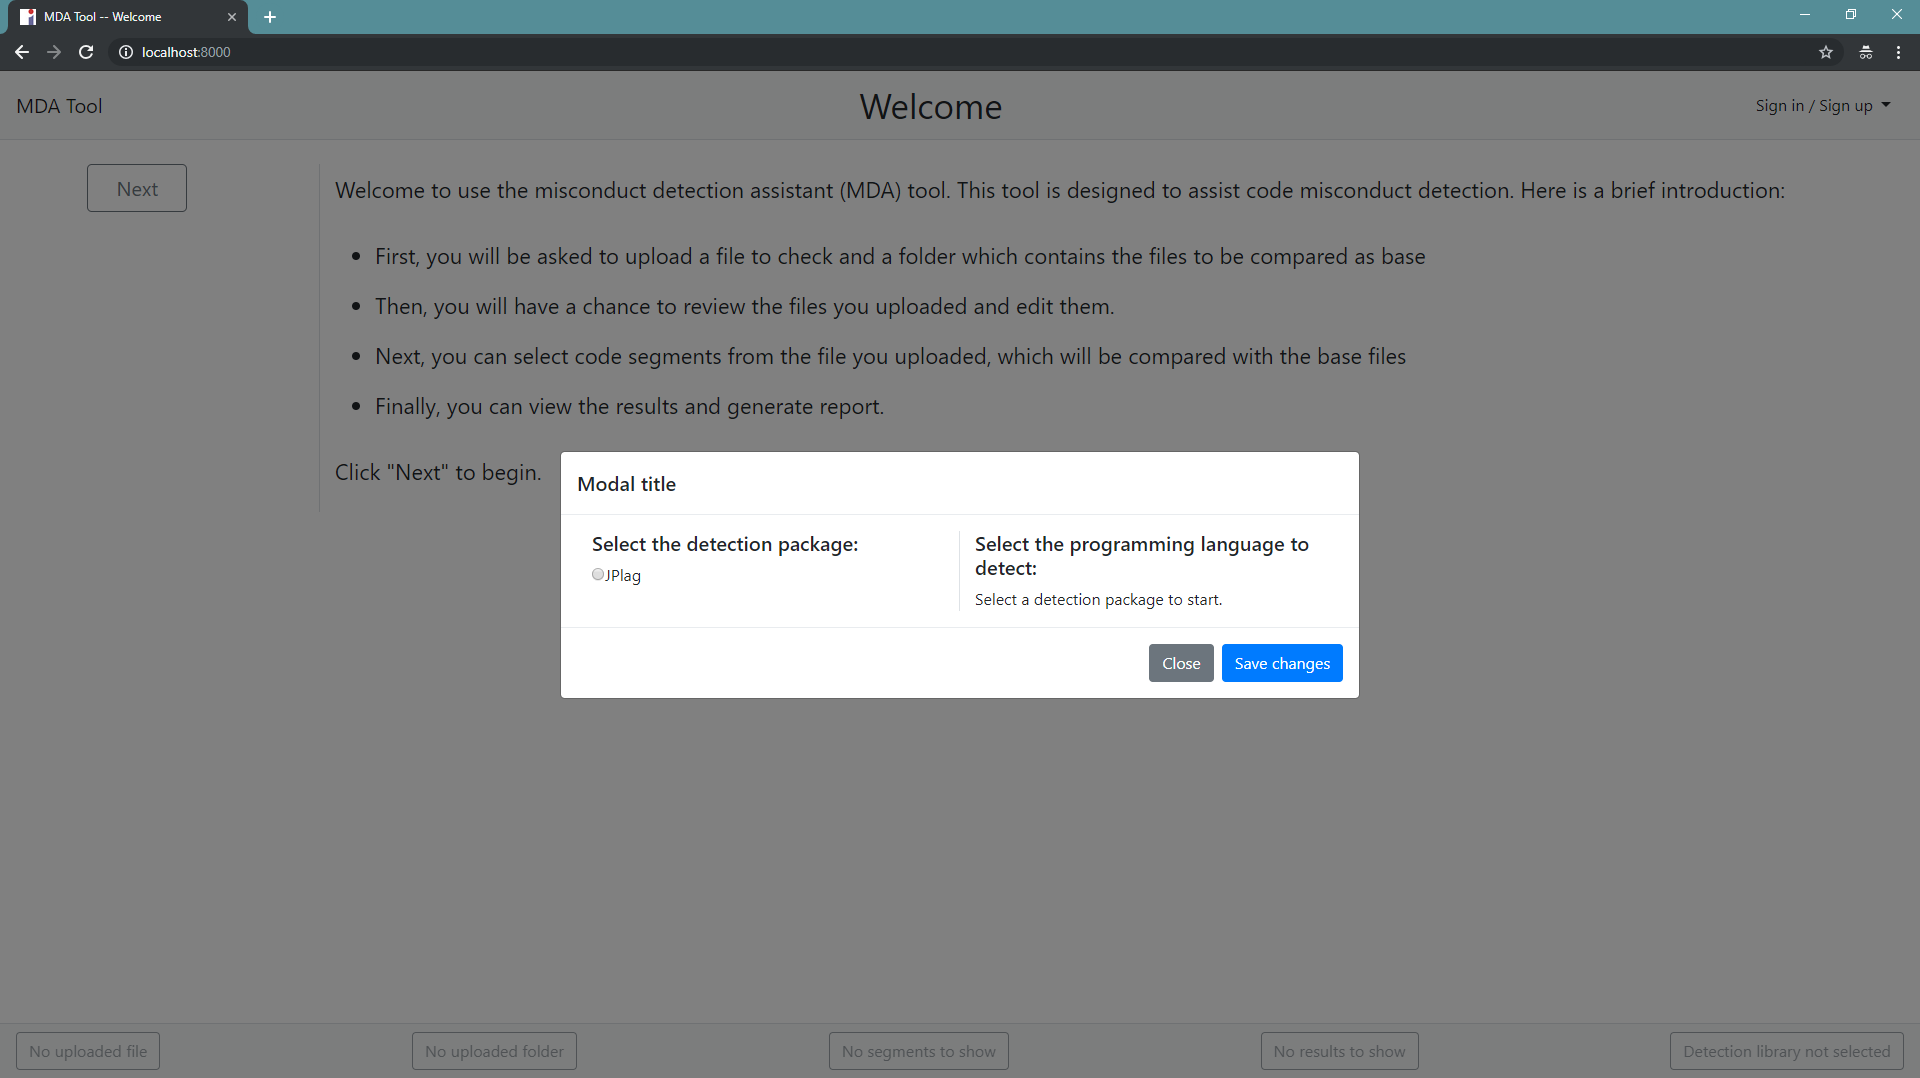
\includegraphics[width=12cm]{img/bug_1-2.png}
\caption{\bugfirst $\ $ Screenshot 2}
\label{fig:bug1_2}
\end{figure}

\begin{figure}[!h]
\centering
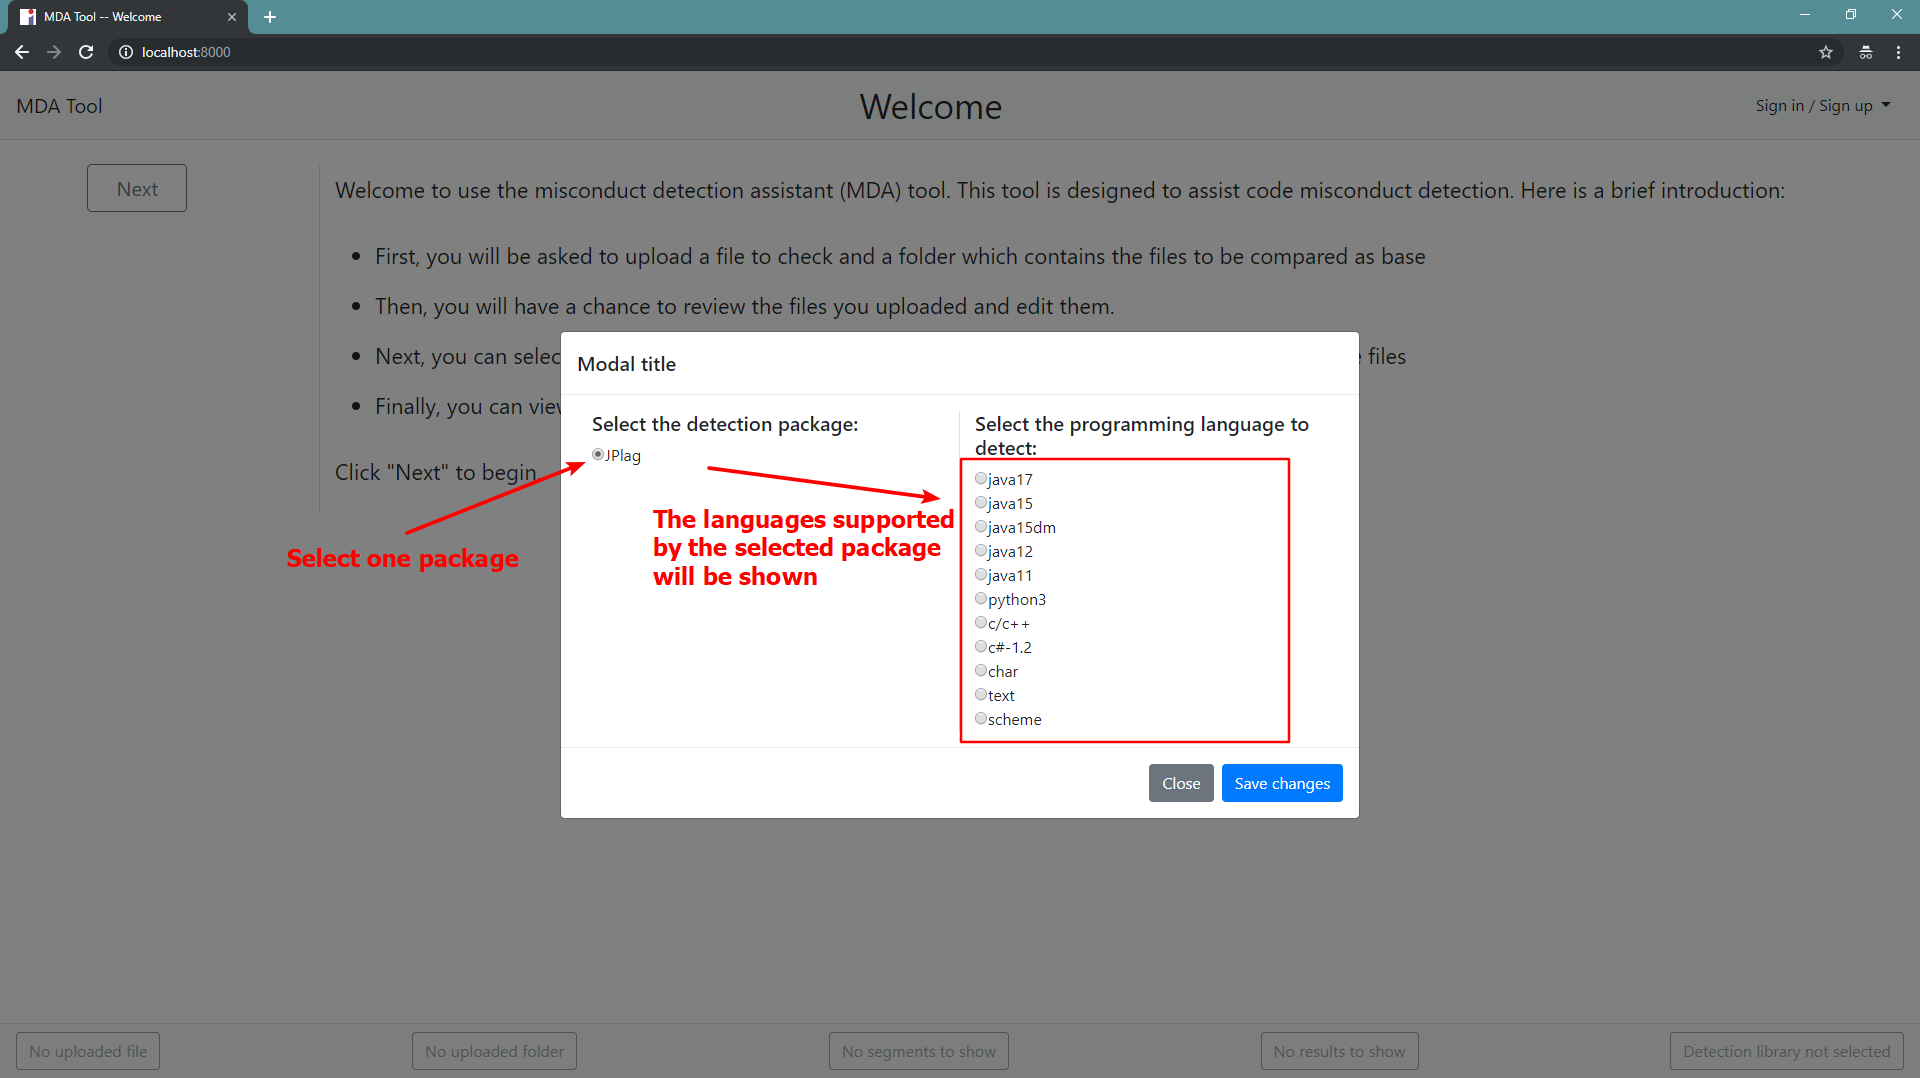
\includegraphics[width=12cm]{img/bug_1-3.png}
\caption{\bugfirst $\ $ Screenshot 3}
\label{fig:bug1_3}
\end{figure}

\begin{figure}[!h]
\centering
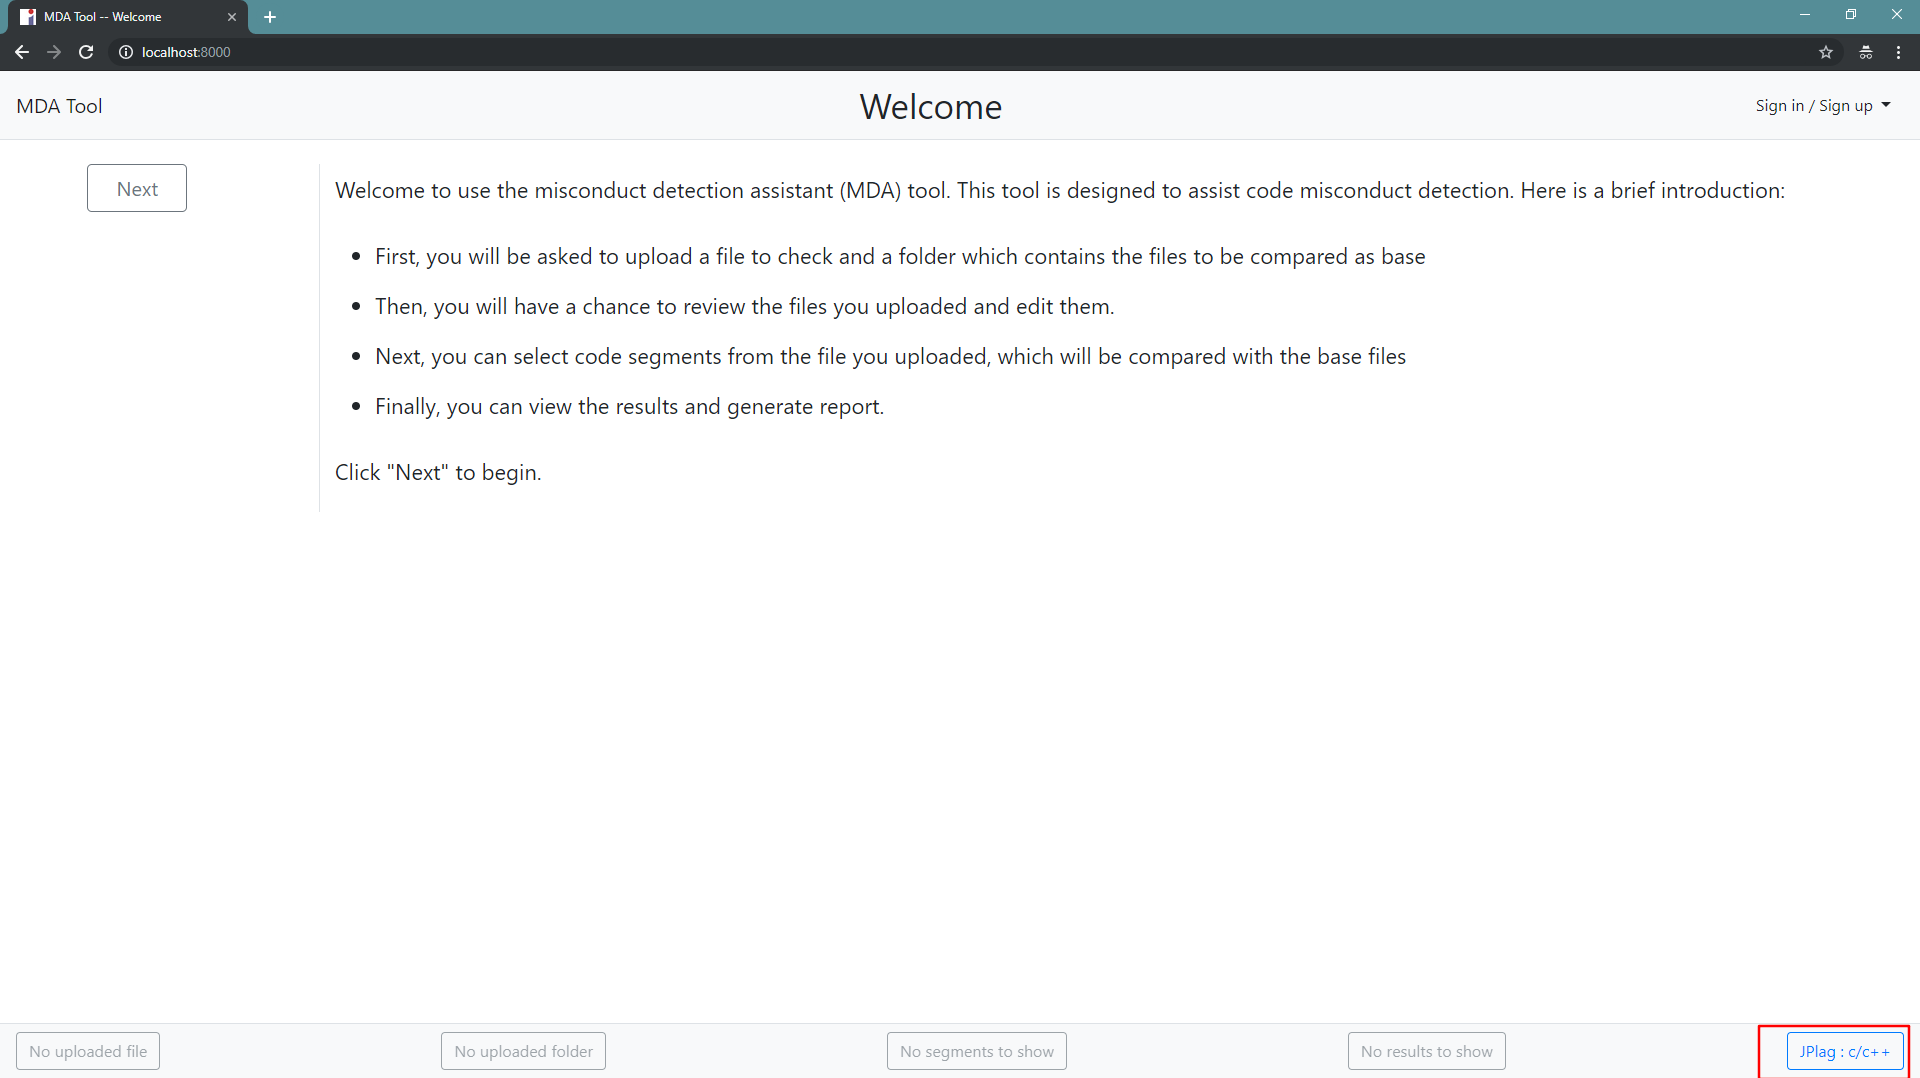
\includegraphics[width=12cm]{img/bug_1-4.png}
\caption{\bugfirst $\ $ Screenshot 4}
\label{fig:bug1_4}
\end{figure}

\clearpage

\begin{figure}[!h]
\centering
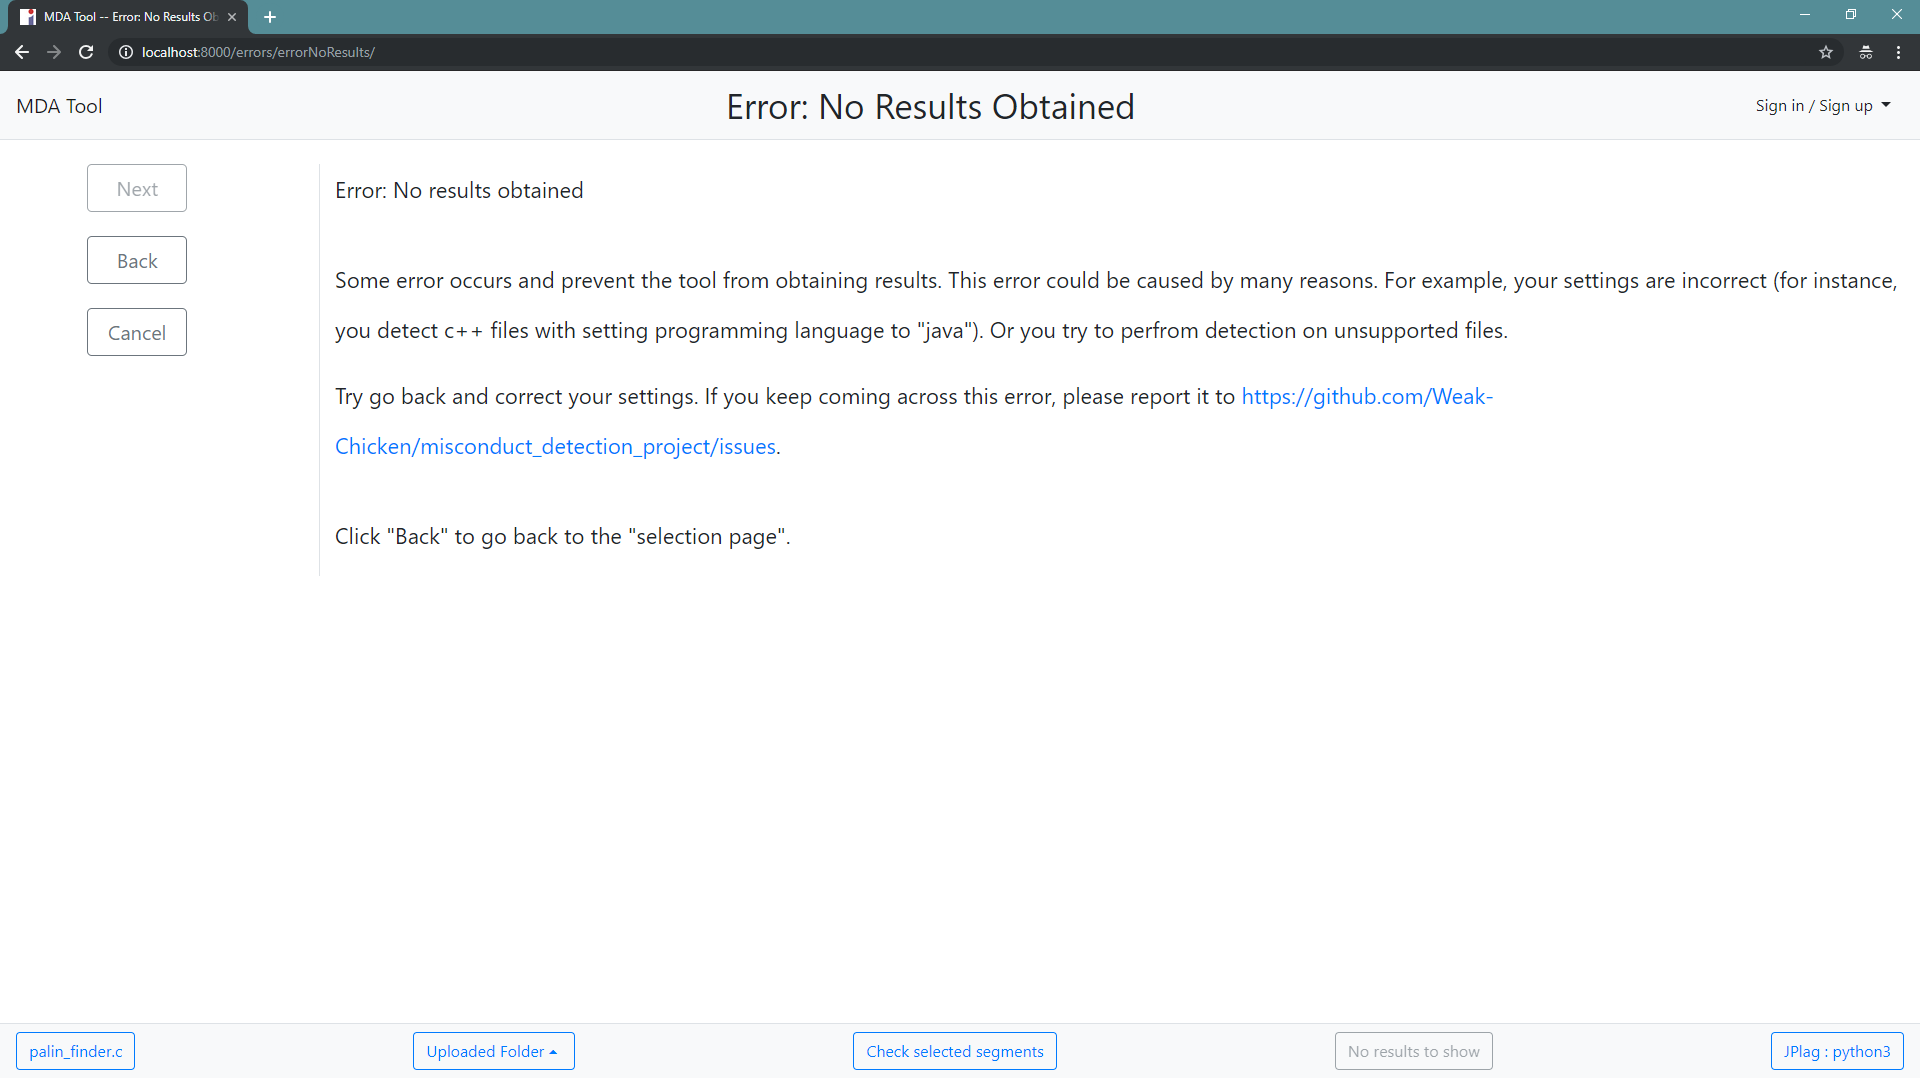
\includegraphics[width=12cm]{img/bug_1-5.png}
\caption{\bugfirst $\ $ Error Page Screenshot 5}
\label{fig:bug1_5}
\end{figure}

Please notice that this error will be shown when the returned results folder is empty. Therefore, there also might be some other errors could raise this error.

\section{Auto Programming Language Selection Function in Use} \label{bug_2_expl}

\begin{figure}[!h]
\centering
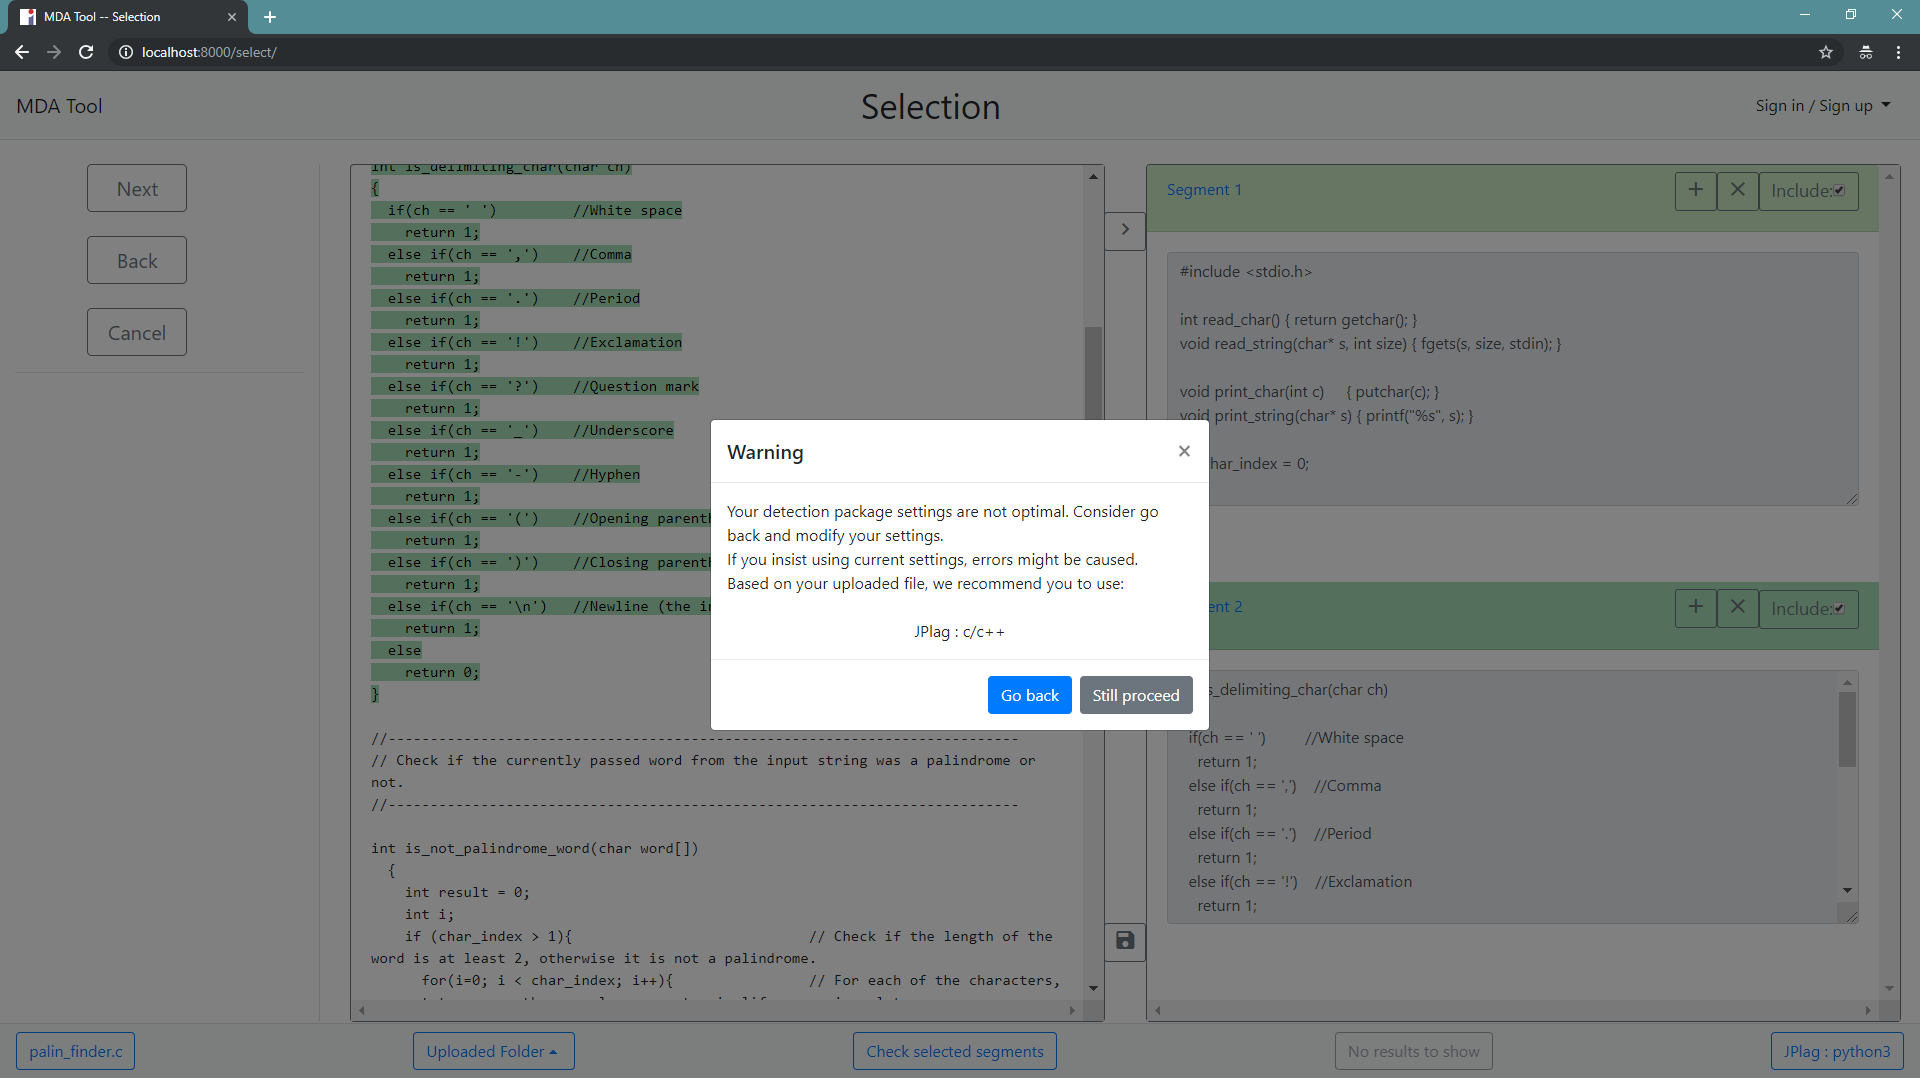
\includegraphics[width=12cm]{img/bug_2-1.png}
\caption{\bugsecond $\ $ Screenshot 1}
\label{fig:bug2_1}
\end{figure}

As shown in Figure \ref{fig:bug2_1}, when the user is not using the optimal settings saved in the server, the auto programming language selection function will give corresponding suggestions and warning to the user. However, the user can ignore the suggestion and still proceed.

If the user has not provided any settings, the function will stop the user from performing detection and require the user to go back and give settings. As shown in Figure \ref{fig:bug2_2}, the \enquote{still proceed} button is unclickable.

\clearpage

\begin{figure}[!h]
\centering
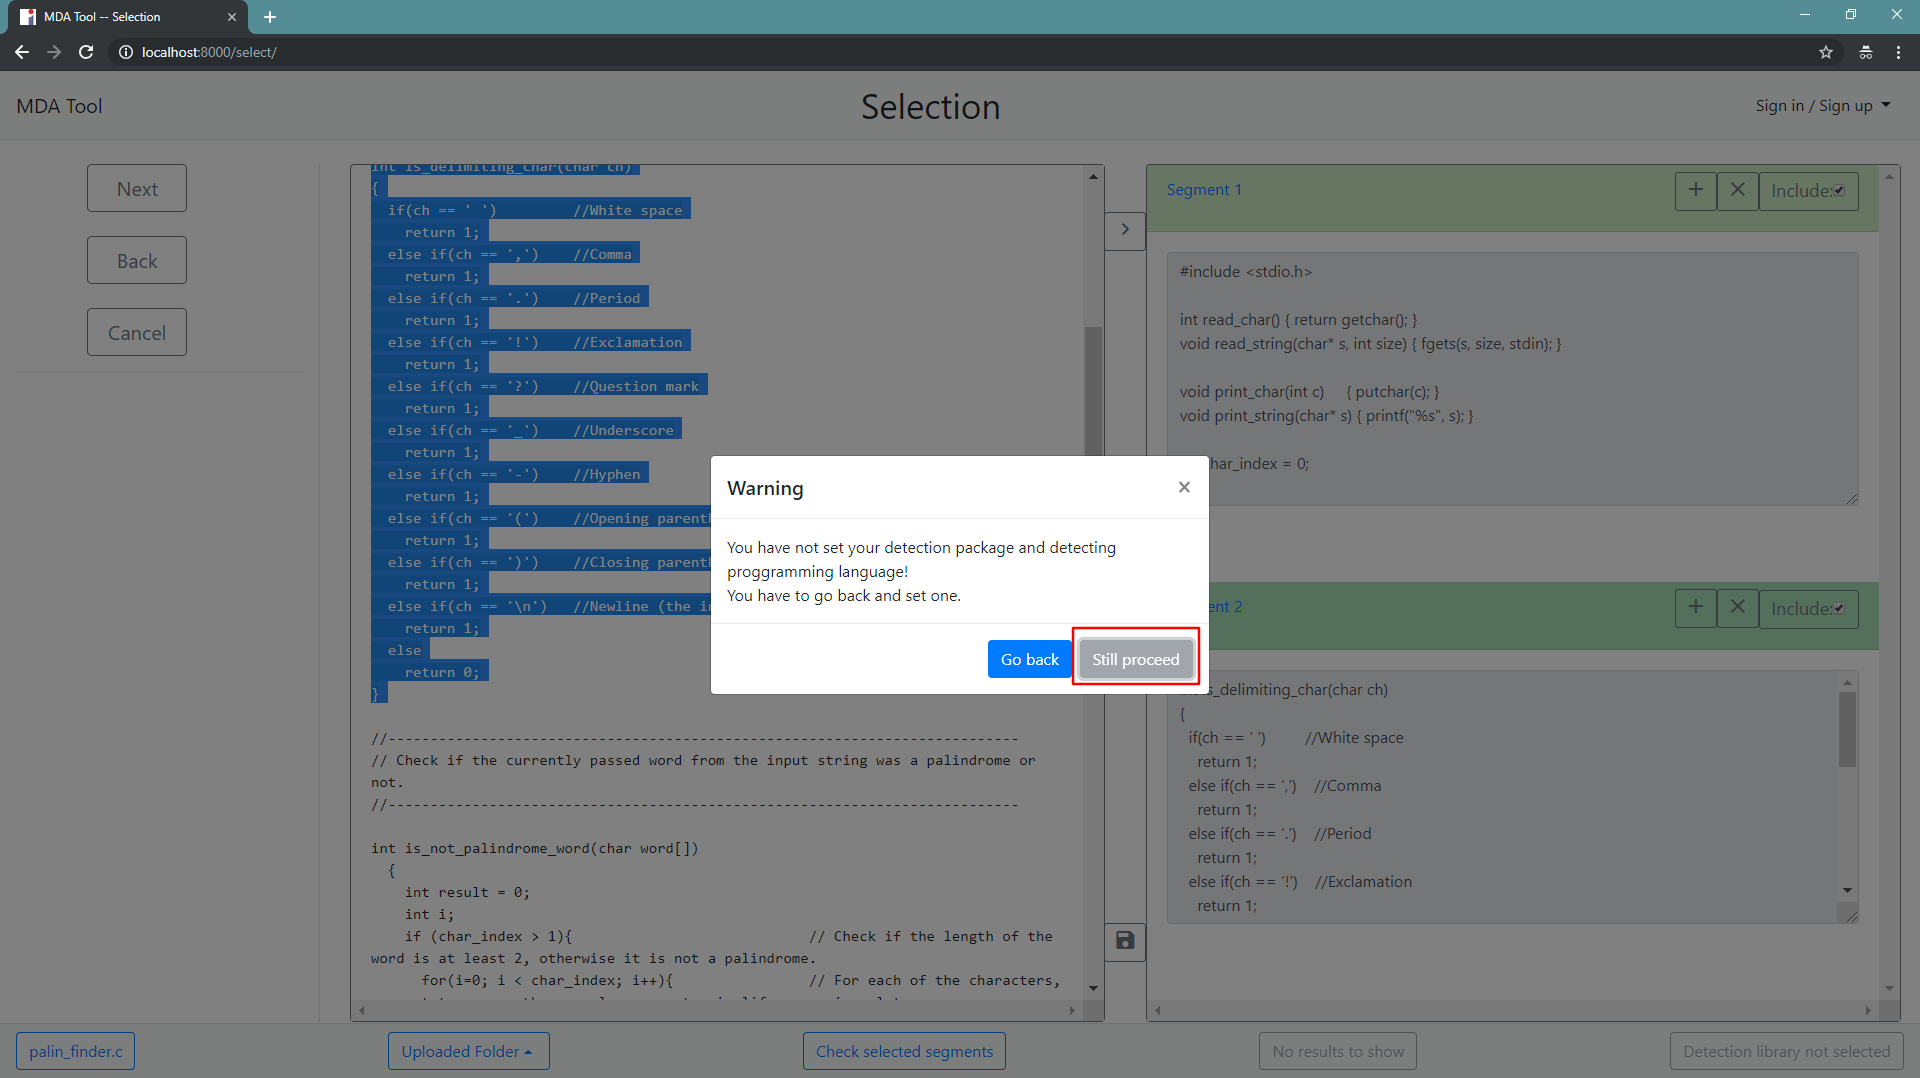
\includegraphics[width=12cm]{img/bug_2-2.png}
\caption{\bugsecond $\ $ Screenshot 2}
\label{fig:bug2_2}
\end{figure}

\printindex

\end{document}
